\chapter{Cheating Even Works on \\ Randomized Data}
\label{ch:fss-randomized}

We can push the example from our previous lesson to the extreme. We will randomize the classification data. We will take the column with the class values and randomly permute it. We will use the Randomize widget to do this.

Later, we will classify this data set. We expect low classification accuracy on randomized data set. Then, we will select five features that are most associated with the class. Even though we randomly permuted the classes, there have to be some features that are weakly correlated with the class. Simply because we have tens of thousands of features, and we have only a few samples. There are enough features to associate with class simply by chance. Finally, we will score a random forest on a randomized data set with selected features.

Compare the scores reported by cross-validation on different data sets in this pipeline. Why is the accuracy in the final one relatively high? Would adding more “most informative features” improve or degrade the cross-validated performance on a randomized data set?

\marginnote{\textbf{\textsf{Instead of selecting the five most informative features, you can further reduce this number. Say, to two most informative features. What happens? Why does accuracy rise after this change?}}}
%
\begin{figure}[h]
    \centering
    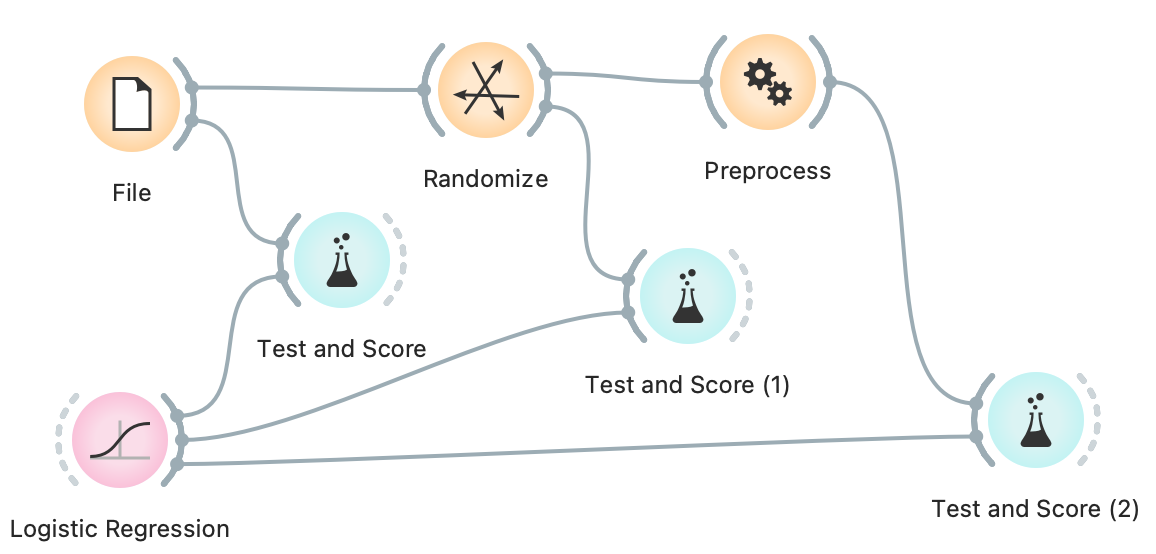
\includegraphics[scale=0.5]{randomize-fss.png}
    \caption{$\;$}
\end{figure}